\chapter{Modelli di Encoding e Decoding Neuronale}

\section{Funzione di risposta neuronale e frequenza di scarica}

Il sistema nervoso interagisce con l'ambiente esterno ricevendo stimoli sensoriali e producendo risposte motorie o cognitive. Comprendere il legame quantitativo tra le caratteristiche fisiche di uno stimolo (come l'intensità di una luce, la frequenza di un suono o la direzione di un movimento) e i potenziali d'azione generati dalle cellule nervose è l'obiettivo centrale dello studio dell'encoding e del decoding neuronale. 

L'\textbf{encoding} (o codifica) è il processo mediante il quale un neurone converte le proprietà di uno stimolo in un segnale elettrico, tipicamente rappresentato da una sequenza temporale di potenziali d'azione, detti \textit{spike}. Formalmente, l'encoding risponde alla domanda: \textit{dato uno stimolo noto, qual è la probabilità che il neurone risponda generando un determinato pattern di spike?}

Il \textbf{decoding} (o decodifica) costituisce invece il processo inverso. L'obiettivo in questo caso è dedurre lo stimolo originario a partire dall'osservazione dell'attività neuronale (il treno di spike). Questa operazione è fondamentale non solo per comprendere come il cervello interpreti i dati sensoriali, ma anche per lo sviluppo di tecnologie biomediche come le interfacce cervello-computer (Brain-Computer Interfaces). 

Trattare il \textbf{legame stimolo-risposta} in modo puramente deterministico è tuttavia impossibile. La sequenza di spike prodotta da un neurone è complessa e riflette molteplici fattori riguardanti la dinamica intrinseca della cellula: l'adattamento, lo stato dei canali ionici, il rumore interno e le fluttuazioni sinaptiche. Spesso si osservano ampie variazioni nella risposta cellulare tra una prova sperimentale (trial) e l'altra, pur mantenendo identico lo stimolo. Pertanto, sia l'encoding che il decoding devono essere affrontati con un approccio \textbf{probabilistico}, stimando la probabilità che si verifichi un certo comportamento neuronale.

\subsection{Treni di Impulsi e Frequenza di Scarica}

Ogni potenziale d'azione ha una durata molto breve e una forma d'onda stereotipata. Ai fini della codifica dell'informazione, la forma dello spike viene spesso trascurata, assimilando l'evento a un impulso puntuale. In una registrazione contenente $n$ spike, identificando con $t_i$ l'istante in cui si verifica l'i-esimo spike in un intervallo di tempo $0 \le t \le T$, l'intero treno di impulsi può essere descritto dalla \textbf{funzione di risposta neuronale} $\rho(t)$, definita tramite la somma di delta di Dirac:
\begin{equation}
\rho(t) = \sum_{i=1}^{n} \delta(t - t_i)
\end{equation}
Questa funzione non misura l'ampiezza elettrica del segnale, bensì l'occorrenza temporale esatta degli eventi.

\subsection{L'Ipotesi della Codifica in Frequenza (Rate Coding)}
L'ipotesi della codifica in frequenza suggerisce che il meccanismo primario utilizzato dal neurone per veicolare informazione sia la sua frequenza di scarica (\textit{firing rate}, indicato con $r$). Secondo questo modello classico (formalizzato già dagli studi di Adrian e Zotterman nel 1926 sulla pressione cutanea nei gatti), maggiore è l'intensità o la rilevanza dello stimolo, maggiore sarà la frequenza con cui il neurone genera potenziali d'azione.

A partire dalla funzione di risposta $\rho(t)$, esistono diverse definizioni per calcolare la frequenza di scarica:

\begin{enumerate}
    \item \textbf{Calcolo sull'intero trial}: Consiste nel contare il numero totale di spike $n$ e dividerlo per la durata del trial $T$. Matematicamente corrisponde alla media nel tempo dell'integrale della risposta:
    \begin{equation}
    r = \frac{n}{T} = \frac{1}{T} \int_{0}^{T} \rho(\tau) \, d\tau \quad \large[Hz]
    \end{equation}
    Pur fornendo una misura semplice (in Hz), questo approccio azzera completamente la risoluzione temporale, rendendo invisibili le variazioni della risposta neurale durante l'esposizione allo stimolo.
    
    \item \textbf{Calcolo locale tempo-variante ($r(t)$)}: Per preservare la dinamica della risposta, l'integrale viene valutato non più sull'intero $T$, ma all'interno di una piccola finestra temporale $\Delta t$:
    \begin{equation}
    r(t) = \frac{1}{\Delta t} \int_{t}^{t+\Delta t} \rho(\tau) \, d\tau
    \end{equation}
    Se $\Delta t$ è molto piccolo, l'affidabilità statistica sul singolo trial crolla (vi sarà al massimo 1 o 0 spike). Per ovviare a questo problema, l'esperimento viene ripetuto più volte (multi-trial) e la risposta viene mediata tra le varie prove, portando alla costruzione del PSTH (\textit{Peri-Stimulus Time Histogram}):
    \begin{equation}
    r(t) = \frac{1}{\Delta t} \int_{t}^{t+\Delta t} \langle \rho(\tau) \rangle \, d\tau
    \end{equation}
    dove il simbolo $\langle \dots \rangle$ indica la media lungo i trial. Il \textbf{PSTH} (\textit{Peri-Stimulus Time Histogram}) è un istogramma che rappresenta la frequenza media di spike (potenziali d’azione) in funzione del tempo rispetto all’inizio di uno stimolo, calcolata su più ripetizioni dello stesso esperimento (i cosiddetti trial)
\end{enumerate}

\begin{figure}[h!]
    \centering
    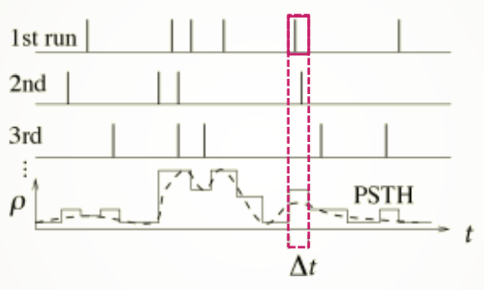
\includegraphics[width=0.5\linewidth]{immagini/multitrial.png}
\end{figure}
\newpage
Moltiplicando il firing rate istantaneo $r(t)$ per un intervallo temporale sufficientemente piccolo $\Delta t$, si ottiene il numero medio di spike attesi in quell'intervallo. Su una base di numerosi trial, $r(t)\Delta t$ esprime la probabilità che uno spike si verifichi in quell'istante:
\begin{equation}
P(\text{spike in } [t, t+\Delta t]) \approx r(t)\Delta t
\end{equation}

\subsection{Metodologie Avanzate per il Calcolo di $r(t)$}

La scelta di come calcolare $r(t)$ determina il compromesso tra risoluzione temporale e regolarità della stima (smoothness). Possiamo identificare quattro approcci principali, basati sull'utilizzo di diverse funzioni di finestratura (kernel). 

Il calcolo della frequenza istantanea può essere generalizzato come l'integrale di convoluzione tra la funzione di risposta $\rho(t)$ e una determinata funzione finestra $\omega(\tau)$ a energia unitaria:
\begin{equation}
r(t) = \int_{-\infty}^{+\infty} \omega(\tau) \rho(t-\tau) \, d\tau = \sum_{i=1}^{n} \omega(t - t_i)
\end{equation}

\begin{itemize}
    \item \textbf{1. Finestra rettangolare fissa}: Si divide l'asse temporale in bin discreti non sovrapposti. Ha il vantaggio di essere semplice da calcolare, ma offre una bassa risoluzione temporale. Assume che all'interno di ogni bin il tasso di scarica sia costante.
    \begin{figure}
        \centering
        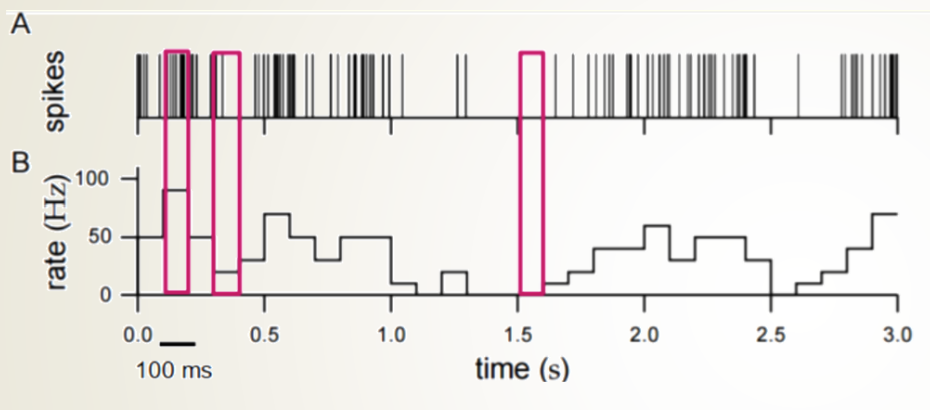
\includegraphics[width=0.5\linewidth]{immagini/rt1.png}
    \end{figure}
    \item \textbf{2. Finestra rettangolare mobile}: Un kernel rettangolare di ampiezza $\Delta t$ viene fatto scorrere in modo continuo lungo l'asse dei tempi. Questo migliora la continuità della curva di $r(t)$, ma genera misure vicine che non sono statisticamente indipendenti, poiché condividono una parte degli spike calcolati.
    \item \textbf{3. Finestra Gaussiana}: Utilizza come funzione $\omega(\tau)$ una Gaussiana a media nulla. Il parametro $\sigma_\omega$ regola l'ampiezza e quindi la risoluzione temporale:
    \begin{equation}
    \omega(\tau) = \frac{1}{\sqrt{2\pi}\sigma_\omega} e^{-\frac{\tau^2}{2\sigma_\omega^2}}
    \end{equation}
    Produce una stima estremamente fluida. Tuttavia, essendo una finestra simmetrica, "guarda" al futuro e al passato dello spike (è un filtro non causale), violando in parte il realismo fisiologico del processo di elaborazione in tempo reale da parte della sinapsi post-sinaptica.
    \item \textbf{4. Finestra Causale}: Utilizza una funzione asimmetrica ($\omega(\tau) = 0$ per $\tau < 0$). Mima più da vicino l'integrazione di membrana post-sinaptica (come la forma di un potenziale post-sinaptico eccitatorio). Sebbene sia la più accurata biologicamente, produce un segnale più asimmetrico e difficile da analizzare matematicamente rispetto alla Gaussiana.
\end{itemize}

\begin{table}[h]
\centering
\begin{tabular}{lp{4cm}p{4cm}}
\toprule
\textbf{Finestra $\omega(t)$} & \textbf{Pro} & \textbf{Contro} \\
\midrule
Rettangolare fissa & Calcolo immediato & Bassa risoluzione temporale \\
Rettangolare mobile & Migliore continuità & Misure fortemente correlate \\
Gaussiana simmetrica & $r(t)$ molto fluida e derivabile & Non causale (non realistica) \\
Filtro Causale & Rispetta la fisiologia cellulare & Matematicamente complessa \\
\bottomrule
\end{tabular}
\caption{Confronto tra le funzioni di finestratura per il calcolo di $r(t)$.}
\end{table}

%%%
\iffalse %%%%%
%%%%

\section{Le Curve di Tuning}

Una \textbf{curva di tuning} descrive l'andamento della risposta media di un neurone, espressa come $\langle r \rangle$, in funzione di una specifica caratteristica $s$ dello stimolo, considerata stazionaria durante ogni prova.

Sperimentalmente, la curva si costruisce facendo variare sistematicamente il parametro $s$ (ad esempio l'angolo visivo, il contrasto o la direzione acustica) lungo diverse ripetizioni. Per ogni valore di $s$, si calcola la frequenza di scarica media sui trial. Infine, i punti sperimentali vengono interpolati mediante una funzione matematica $f(s)$ che modella la capacità del neurone di "sintonizzarsi" su determinati parametri fisici.

Esempi classici di curve di tuning includono:
\begin{enumerate}
    \item \textbf{Neuroni della corteccia visiva primaria (orientamento)}: Rispondono in maniera selettiva a barre luminose presentate in determinati angoli. La curva di tuning assume spesso una forma Gaussiana:
    \begin{equation}
    f(s) = r_{max} e^{-\frac{1}{2}\left(\frac{s-s_{max}}{\sigma_f}\right)^2}
    \end{equation}
    dove $s_{max}$ è l'angolo preferito che evoca la scarica massima $r_{max}$, e $\sigma_f$ determina la selettività (la "larghezza" della sintonizzazione).
    
    \item \textbf{Neuroni della corteccia motoria primaria (direzione)}: La frequenza di scarica modula in base all'angolo del movimento compiuto da un arto. L'adattamento segue generalmente una legge del coseno:
    \begin{equation}
    f(s) = r_0 + (r_{max}-r_0)\cos(s-s_{max})
    \end{equation}
    dove $r_0$ fornisce un offset di frequenza a riposo.
    
    \item \textbf{Neuroni per la disparità retinica binoculare}: Implicati nella percezione della profondità spaziale, mostrano una transizione repentina (a gradino o sigmoide) in corrispondenza del passaggio dalla disparità negativa a quella positiva:
    \begin{equation}
    f(s) = \frac{r_{max}}{1+\exp[(s_{1/2}-s)/\Delta_s]}
    \end{equation}
    Questo modello indica l'esistenza di una soglia netta di attivazione rispetto alla posizione degli oggetti osservati in tre dimensioni.
\end{enumerate}

\section{Fondamenti del Decoding Neuronale e Probabilità}

Nel decodificare una risposta neuronale ci affidiamo all'uso della probabilità condizionata. L'encoding determina la probabilità $P[r \mid s]$ (la probabilità di registrare il tasso di scarica $r$ se l'ambiente presenta lo stimolo $s$). Il decoding, mediante l'inversione Bayesiana, indaga invece la $P[s \mid r]$: ricevendo un segnale di frequenza $r$, qual è lo stimolo $s$ che ha massimizzato tale probabilità?

Si consideri un classico esperimento di discriminazione visiva in cui si richiede di indicare la direzione globale di punti in movimento su uno schermo. Lo stimolo possiede due livelli di direzione (positiva +, che coincide con la preferenza del neurone, e negativa -). Un parametro cruciale è la \textbf{coerenza} del movimento: quando essa è del 100\%, tutti i punti si muovono all'unisono; allo 0\%, il moto è totalmente casuale e dominato dal rumore visivo.

Registrando il tasso di scarica $r$ del neurone a vari livelli di coerenza per entrambe le direzioni, possiamo generare due distribuzioni statistiche: $P[r \mid +]$ e $P[r \mid -]$. Assumendo che si tratti di distribuzioni gaussiane con medie distinte $\langle r \rangle_+$ e $\langle r \rangle_-$ ma varianza comune $\sigma_r^2$, possiamo definire l'indice di discriminabilità $d'$:
\begin{equation}
d' = \frac{\langle r \rangle_+ - \langle r \rangle_-}{\sigma_r}
\end{equation}
Maggiore è la coerenza dello stimolo, maggiore sarà l'allontanamento tra le due medie e, conseguentemente, l'elevato valore di $d'$, garantendo un decoding facile e accurato.

\subsection{Classificazione a Soglia}
Per operare effettivamente la discriminazione, il decoder matematico deve introdurre una soglia decisionale $z$.
Se $r \ge z$, lo stimolo è classificato come direzione (+).
Se $r < z$, lo stimolo è classificato come direzione (-).
Scegliere la corretta posizione della soglia $z$ lungo l'asse delle ascisse è un problema di ottimizzazione. Valutando le probabilità relative alla posizione di $z$, generiamo i classici indici diagnostici:
\begin{itemize}
    \item \textbf{Vero Positivo (TP)}: $\beta(z) = P[r \ge z \mid +]$ (direzione + corretta).
    \item \textbf{Falso Positivo (FP)}: $\alpha(z) = P[r \ge z \mid -]$ (direzione - confusa per +).
    \item \textbf{Vero Negativo (TN)}: $1 - \alpha(z) = P[r < z \mid -]$ (direzione - corretta).
    \item \textbf{Falso Negativo (FN)}: $1 - \beta(z) = P[r < z \mid +]$ (direzione + ignorata).
\end{itemize}

\section{Accuratezza e Curve ROC}

In ambito clinico e neuroscientifico, il compromesso tra l'identificazione corretta di eventi rari e l'evitamento dei falsi allarmi è studiato mediante la Sensibilità (\textit{True Positive Rate}, TPR) e la Specificità (\textit{True Negative Rate}, TNR). 
\begin{equation}
\text{TPR} = \frac{\text{TP}}{\text{TP} + \text{FN}}, \quad \text{TNR} = \frac{\text{TN}}{\text{TN} + \text{FP}}, \quad \text{FPR} = 1 - \text{TNR}
\end{equation}

La \textbf{curva ROC} (\textit{Receiver Operating Characteristic}) è un grafico in cui viene tracciato il TPR in funzione del FPR (cioè Sensibilità contro $1 - \text{Specificità}$) per ogni valore possibile della soglia $z$.
\begin{itemize}
    \item Se $z = 0$, tutti gli eventi cadono nella classe positiva (FPR=1, TPR=1).
    \item Se $z \to \infty$, nessun evento è classificato come positivo (FPR=0, TPR=0).
    \item Una curva coincidente con la diagonale corrisponde a un classificatore casuale (nessun guadagno predittivo, prestazioni del 50\%).
    \item Una classificazione perfetta genererebbe un punto nelle coordinate (0,1).
\end{itemize}

L'area sottesa dalla curva ROC si chiama \textbf{AUC} (\textit{Area Under Curve}). Fornisce un punteggio scalare, indipendente da una specifica soglia, che varia tra $0.5$ (caso pessimo) e $1.0$ (predizione perfetta). Statisticamente, l'AUC rappresenta la probabilità che il classificatore assegni un valore di funzione (nel nostro caso un firing rate) superiore a un'istanza positiva presa a caso rispetto a una negativa.

Applicando l'analisi ROC ai trial neurofisiologici precedentemente discussi (l'esperimento della direzione di movimento dei punti a diverse coerenze), si nota che l'AUC della risposta di un singolo neurone della corteccia visiva (misurata matematicamente) si sovrappone in maniera sorprendente alla curva psicometrica del comportamento manifesto del soggetto. In termini semplici, l'informazione codificata nella frequenza di scarica di una singola cellula è sufficiente per spiegare le decisioni motorie e percettive dell'organismo. 

\section{Conclusioni e Prospettive Cliniche}

Il modello a soglia dimostra che un decoder biologico o artificiale può sfruttare la sola frequenza statistica per interpretare il mondo in presenza di rumore. Tuttavia, si tratta di un costrutto puramente matematico e descrittivo: non considera l'architettura biologica reale delle reti cerebrali, l'integrazione di centinaia di migliaia di sinapsi o le complesse tempistiche elettrochimiche, che andrebbero investigate tramite modelli a rete più evoluti.

Ciononostante, i risultati dell'analisi del decoding hanno generato applicazioni di portata storica nella riabilitazione medica. L'acquisizione di segnali da \textit{microelectrode arrays} impiantati nel cervello permette ai computer di applicare modelli statistici e reti neurali in tempo reale. Dedurre le traiettorie motorie tridimensionali (3D arm trajectory) dal firing rate di una popolazione di cellule è il principio cardine delle \textbf{Brain-Computer Interfaces} e delle neuroprotesi. Elaborando gli spike isolati dal rumore di fondo, i decoder neuronali permettono ai pazienti con deficit motori severi di tradurre l'intento cerebrale direttamente nel controllo cinetico di bracci robotici, creando un ponte ingegneristico lì dove la biologia ha interrotto la comunicazione naturale.
\fi